\documentclass[a4paper]{article}
\usepackage{geometry}
\geometry{left=2.5cm,right=2.5cm,top=2cm,bottom=2.5cm}
\usepackage[pdftex]{graphicx}

\title{NoSQL database}
\author{Xinyang Li A53209370,Che Liu A53209595}
\date{}
\begin{document}
\maketitle %
\section{Introduction}
In this project we are asked to build the storage underlying a NoSQL database. We find the requirement is very similar to the google big-table and the LevelDB implementation. Therefore, we use part of ideas from the two papers and build our own database version.
This is not the traditional database but it is still not a NoSQL database.
The second section discussed about our own architecture of this database, section 3 discussed about how we implement the action required, including append, read, write data and join, select from table. Section 4 discussed about our simple test and how to measure time. Section 5 is a short conclusion.
\section{Architecture}
\subsection{layers}
The database has three layers:\\
The first layer is the class for users to create the whole database. Users can use API of this level to create tables, append, edit and delete data, and join, select tables. We do not have the time to realize a query engine, so in this case we just offer some functions to users to do those actions. In this layer, all tables are managed under this big class. One class represents one database. We choose this implementation because we do not want users to take care about the communication of tables. The users only know the id of tables and then do the action.\\
The second layer is the storage component in the memory. It is formed by two components. The first component is to manage the table action. This component, like the graph shows, is to provide the transformation from row store to the column-orientated store. The API of this component to the database are still based on rows and we use the component to traverse it into columns. The second component of this layer handles each columns. It contains a memTable to store the recent information, several immutable table to store the recent information for the quick search. Once the memTable store too many key-value pairs, those pairs will be stored to the immutable table and once the immutable table is too large, we do a minor compaction to pack the immutable table and send it to the third layer, where control the disk.
The third layer is all thing about the disk. This layer received package from top layer and store them. Once the files are too much, we do major compaction and sort them all. We use json as SSTable in this layer. In this layer, every record is to set the value. The set action here is a record, and the delete action here is to set the value to None.
\\
  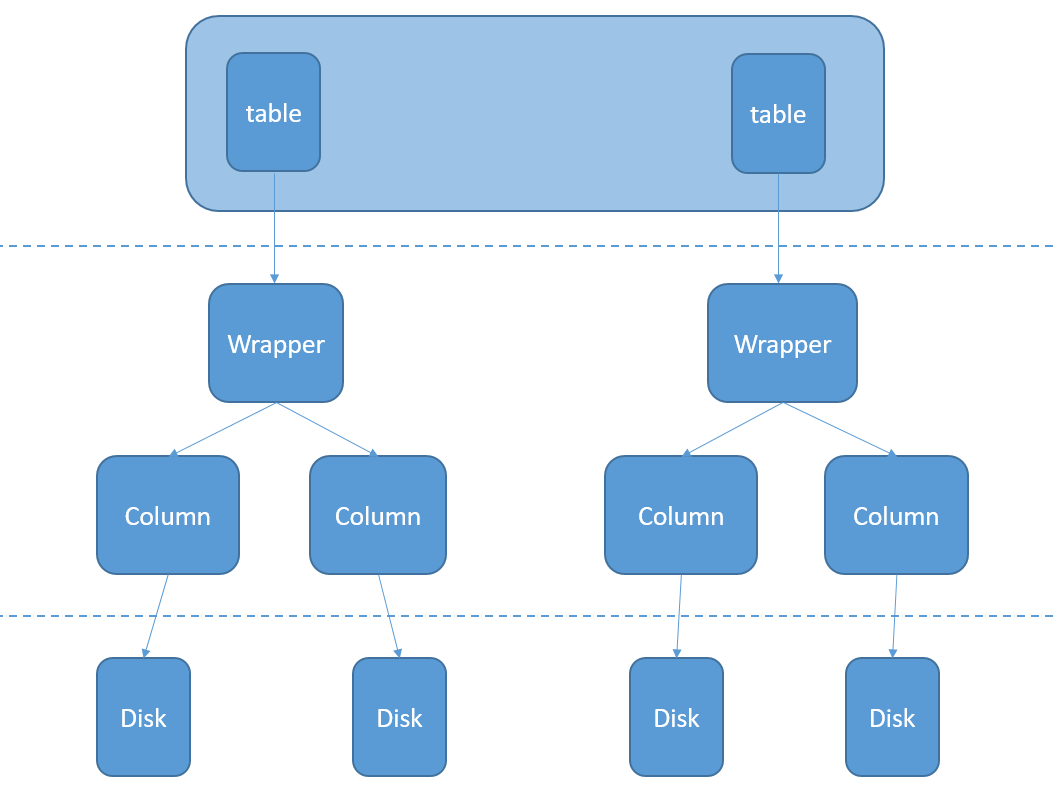
\includegraphics[width=1.0\linewidth]{cse291-1.png}\\
\subsection{connection APIs}
In the first layer we provide APIs to users. It include create table, append data, delete a key, select, and join tables.\\
In the wrapper we provide APIs to the database, the database can use append/delete to modify data in specific columns, get the whole data of one column and find the recent update of a key on one column.\\
In the column, we provide APIs to wrapper. Since there is one column manage for one column. We do not need to specify the column name. We just do get, edit by key, get all the data.\\
In the last column, we provide only two APIs: save file, and get file.\\


\section{Implementation of Action}
In this section we are going to explain how we implement those action required.
\subsection{append, edit, delete data}
For append and edit action, we use "set" to do this function. the set function take the table number and the key number to identify, plus a dictionary to indicate that which column does user want to set. Consider there is a table 1 and the column is name and birthday. And we want to set the name to "aa". What we do here is use the set function: set(1,key,{"name": "aa"}). The difference of append and edit is the completeness. In the edit function, the user can update only part of the column. Since we use column-based storage, the columns are stored separately. And it is reasonable to allow the user to update only part columns. However, the append is different. We need to make sure that every column contains all keys so we can maintain the consistency. So if the user want to append a record, we suggest it give us the values of all columns. If they do not do it, we will set the default value as an empty string. And for the delete action, obviously we need to delete the key in all columns. So there is no need the user indicate the columns, the database will set the value of every column to the None. To notice that, there is a difference between None and empty string. The empty string
\subsection{select, join, where}
For the select and join action, we need to scan all the table. At first, we think about that for every select/join we need to shuffle the storage, which means doing compaction and update every key to the newest. But later we find that necessary. We can join or select on records from old to new, in this way, the data maintain in order and we can let the new table to take care about the  compaction problem. In total, the join action is to join the record, not the special data. Let see if there are two tables: table A and table B. What we do is to take the table A and get all record. For every record, we find if the key is in the table B, if it is, we extract all data of that key and just put the record in the new database. And there is why we need to add record to all column, that is because we need to check the key to see if it is in the database. We do not have the global key, we can only pick up one column and do the check. And the select action is the same. We select the record rather that the true data. We never do the data shuffle and compaction ourselves. Only the disk manage determine the time of compaction. As for the where function, since we do not have the time to implement query engine. So the where is implemented as a function and it only support choose on keys.
\subsection{store in the memory}
The store in memory has nothing to do with the database management. After the column management, the memory store only need to deal with the bunch of key-value pairs. So we do this kind of things: if the value is None and the key has already in the map, we delete the key, if not, we add the None as record. The other things, we just add the record to the map. Once the size of the map is large enough, we pack the map and move it to an immutable table, and we make the map empty. Here is the difference between bigtable and the levelDB. The bigtable pack the memory cache and store them in the disk as some small file and use the minor compaction to merge them. The levelDB introduce the immutable table. This immutable table is in the memory and can only be read. So it only provide the search convinience. My best guess is that LevelDB focus on the performance but the bigtable consider about the scale problem. Bigtable uses all memory as cache so it can achieve better performance on frequent modification. Anyway, we use the idea of immutable table here so we can have better performance when select and join.
\subsection{compaction}
\subsection{bloom filter}
\subsection{compression}
\subsection{store on the disk}

\section{Test}
\end{document}
